\documentclass[border=8pt]{standalone}
\usepackage{tkz-euclide}
\begin{document}
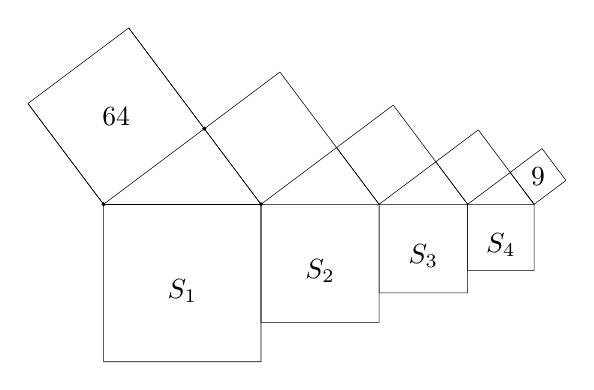
\begin{tikzpicture}[scale=0.2]
	\tkzDefPoints{0/0/A,10/0/B}
	\tkzDefPoints{5/0/M,8/0/N}
	\tkzDrawPoints[color=black,size=1pt](A,B)
	\tkzDrawSegment(A,B)
	\tkzDefPointBy[homothety=center A ratio 7/4](B)
	\tkzGetPoint{C}
%	\tkzDrawPoints[color=black,size=1pt](C)
%	\tkzDrawSegment(B,C)
	%\draw (A)++(0,-0.5) node {$A$};
%	\draw (B)++(0,-0.5) node {$B$};
%	\draw (C)++(0,-0.5) node {$C$};
	\tkzDefPointBy[homothety=center B ratio 7/4](C)
	\tkzGetPoint{D}
%	\tkzDrawPoints[color=black,size=1pt](D)
%	\tkzDrawSegment(C,D)
	%\draw (D)++(0,-0.5) node {$D$};
	\tkzDefPointBy[homothety=center C ratio 7/4](D)
	\tkzGetPoint{E}
%	\tkzDrawPoints[color=black,size=1pt](E)
%	\tkzDrawSegment(D,E)
	%\draw (E)++(0,-0.5) node {$E$};
	\tkzDefPointBy[rotation in rad=center A angle -pi/2](B)
	\tkzGetPoint{A1}
	%\tkzDrawSegment(A,A1)
	\tkzDefPointBy[rotation in rad=center B angle pi/2](A)
	\tkzGetPoint{A2}
%	\tkzDrawSegment(B,A2)
	\tkzDrawPolygon(A,B,A2,A1)
	\tkzDefPointBy[rotation in rad=center B angle -pi/2](C)
	\tkzGetPoint{B1}
	
	\tkzDefPointBy[rotation in rad=center C angle pi/2](B)
	\tkzGetPoint{B2}
	
	\tkzDrawPolygon(B,B1,B2,C)
	
	\tkzDefPointBy[rotation in rad=center C angle -pi/2](D)
	\tkzGetPoint{C1}
	
	\tkzDefPointBy[rotation in rad=center D angle pi/2](C)
	\tkzGetPoint{C2}
	
	\tkzDrawPolygon(C,C1,C2,D)
		\tkzDefPointBy[rotation in rad=center D angle -pi/2](E)
	\tkzGetPoint{D1}
	
	\tkzDefPointBy[rotation in rad=center E angle pi/2](D)
	\tkzGetPoint{D2}
	
	\tkzDrawPolygon(D,D1,D2,E)
%%%%%%%%%%%%%%%%%%%%%%%%%%%%%%%%%%%%%%%%%%%%%%%%%%%%%%%%%%%%
%\tkzDrawPoints[color=red,size=4pt](A2) \tkzDrawSegment(A,A2)
%\tkzDrawPoints[color=blue,size=4pt](A1) \tkzDrawSegment(B,A1)
%\tkzInterLL(A,A2)(B,A1)
\tkzDefMidPoint(A,A2)
\tkzGetPoint{P}
%	\tkzDrawPoints[color=blue,size=1pt](P)
		\draw (P)++(0,-0.5) node {$S_{1}$};
\tkzDefMidPoint(B,B2)
\tkzGetPoint{P1}
%\tkzDrawPoints[color=blue,size=1pt](P1)
\draw (P1)++(0,-0.5) node {$S_{2}$};		
\tkzInterLL(C,C2)(D,C1)
\tkzGetPoint{P2}
%\tkzDrawPoints[color=blue,size=1pt](P2)
\draw (P2)++(0,-0.5) node {$S_{3}$};			
\tkzInterLL(D,D2)(E,D1)
\tkzGetPoint{P3}
%\tkzDrawPoints[color=blue,size=1pt](P3)
\draw (P3)++(0,-0.5) node {$S_{4}$};				
		
%%%%%%%%%%%%%%%%%%%%%%%%%%%%%%%%%%%%%%%%%%%%%%%%%%%%%%%%%%%%		
	\tkzInterCC(M,A)(A,N)
	\tkzGetPoints{A1'}{A2'}
	
\tkzDrawPoints[color=black,size=1pt](A2')
\tkzDefPointBy[rotation in rad=center A angle pi/2](A2')
\tkzGetPoint{A21}
\tkzDrawSegment(A,A21)
\tkzDefPointBy[rotation in rad=center A2' angle -pi/2](A)
\tkzGetPoint{A22}
\tkzDrawSegment(A2',A22)
	\tkzDrawPolygon(A,A2',A22,A21)
\tkzDrawSegment(B,A2')	
\tkzDefPointBy[rotation in rad=center B angle -pi/2](A2')
\tkzGetPoint{B21}
\tkzDefPointBy[rotation in rad=center A2' angle pi/2](B)
\tkzGetPoint{B22}
	\tkzDrawPolygon(B,A2',B22,B21)
\tkzDrawSegment(C,B21)		
\tkzDefPointBy[rotation in rad=center C angle -pi/2](B21)
\tkzGetPoint{C21}
\tkzDefPointBy[rotation in rad=center B21 angle pi/2](C)
\tkzGetPoint{C22}
\tkzDrawPolygon(C,C21,C22,B21)	
\tkzDrawSegment(D,C21)	
\tkzDefPointBy[rotation in rad=center D angle -pi/2](C21)
\tkzGetPoint{D21}
\tkzDefPointBy[rotation in rad=center C21 angle pi/2](D)
\tkzGetPoint{D22}
\tkzDrawPolygon(D,D21,D22,C21)	
\tkzDrawSegment(E,D21)
\tkzDefPointBy[rotation in rad=center E angle -pi/2](D21)
\tkzGetPoint{E21}
\tkzDefPointBy[rotation in rad=center D21 angle pi/2](E)
\tkzGetPoint{E22}
\tkzDrawPolygon(E,E21,E22,D21)

%%%%%%%%%%%%%%%%%%%%%%%%%%%%%%%%%%%%%%%%%%%%%%%%%%%%%%%%	
\tkzInterLL(A,A22)(A2',A21)
\tkzGetPoint{U1}
%\tkzDrawPoints[color=blue,size=1pt](U1)
\draw (U1)++(0,-0.05) node {$64$};

\tkzInterLL(D21,E21)(E,E22)
\tkzGetPoint{U2}
%\tkzDrawPoints[color=blue,size=1pt](U2)
\draw (U2)++(0,0.005) node {$9$};	
\end{tikzpicture}	

\end{document}